\section{Methodology}
\label{s:semantic-closeness}

In this work we aim to utilize information from the semantic behavior of \cnc to
better control and guide the refinement process producing higher quality \abs
while retaining concrete soundness. 

In particular, we define a \textit{semantic
closeness metric} that captures how close the semantic-behavior of two 
neurons are (Section \ref{s:semantic-closeness}). We utilise this semantic
closeness metric to arrange the merge
operations into a tree where lower quality merges involving semantically far
neurons appear higher and can be refined with higher priority (Section
\ref{s:tree}). 

Using this tree we build a framework where refinement can
be done by making cuts of this tree, while still providing concrete soundness
guarantees (Section \ref{s:refinement}). We show that
the merges retained in this refinement process is optimal with respect to the
semantic information (Section \ref{s:optimal-tree}).
This allows us to avoid restoring large number of single neurons(see Section
\ref{s:nn-sam}) and lets us retain merge operations of higher quality. Thus, we
produce an \abs of the desired quality with a much smaller size. 

%While the choice of which nodes to leave merged together is guided by the cuts
%of the tree, the weights attached to the abstract nodes are still chosen
%by following the procedures from Section \ref{s:nn-sam} and \cite{cegar-nn}.
%Thus, the concrete soundness guarantees still hold for the \abs obtained.
%\dmcmt{This point is repeated in \ref{s:refinement}, but this should be okay
%right?}

%In the following sections we describe a general framework for such a unified
%syntactic and semantic refinement process, describing each component in detail.

Using these components, we propose a general abstraction-refinement loop based
framework (Section \ref{s:abs-ref-fw}) that combines syntactic merge operation
with semantic behavior. This framework is able to utilise \gencex from any
source and continually refine until a \abs of desired quality is achieved.

\subsection{Semantic Closeness Factor}
\label{s:semantic-closeness}

\todo{If we are able to get the characterestic based exps run, we can talk
    about that as well.
}

To guide the semantic abstraction process, we define a \textit{semantic
closeness metric} $\cls$: $\cls(\nr{i_1}{l}, \nr{i_2}{l})$ is function that
takes two neurons $\nr{i_1}{l}$ and $\nr{i_2}{l}$ in
the same layer $l$, and returns a real number that
captures how close the behaviors of $\nr{i_1}{l}$ and $\nr{i_2}{l}$ are from a
semantic point of view. The number returned by $\cls$ should be smaller for
neurons whose semantic behavior is closer. Intuitively, this metric would
characterise the semantic behavior of the
neurons in layer $l$ relative to each other, and prioritise certain merges over
others. 

Depending on the application, the precise definition of this metric may be
chosen in various ways. We note that our framework is agnostic to the particular
choice of semantic metric, and a concrete soundness guarantee holds for any such
choice. Inspired by \cite{deep-abstract}, in we chose as the
semantic closeness metric how close the functions computed by the two neurons
are: $||\nrf{i_1}{l} - \nrf{i_2}{l}||$. 

However, since $\nrf{i_1}{l}$ and $\nrf{i_2}{l}$ are functions, computing
$||\nrf{i_1}{l} - \nrf{i_2}{l}||$ precisely is not feasible.
Therefore, we estimate it using a sample set of inputs $X$: $||\ob{i_1}{l}($X$)
- \ob{i_2}{l}($X$)||_2$. This $X$ may be chosen in many ways, for example, it
may be a set of randomly chosen input values satisfying $P$ when
abstracting with respect to a query $(P, \mcnc, Q)$
(Section \ref{s:exp-mnist-rob}), or a dataset when attempting to find a
safe compression (Section \ref{s:exp-mnist-comp}).

\subsection{Tree of Merges}
\label{s:tree}

We use $\cls$ to create a tree structure to prioritise merges wherein leaf nodes
represent the original neurons, and 
non-leaf nodes represent merge operations. The construction of the tree 
follows a bottom-up approach, starting from individual neurons, 
greedily performing the merge operation involving the most similar groups of
neurons, and delaying the merging of dissimilar ones. The resulting tree
captures an optimal ordering of merge operations (Section \ref{s:optimal-tree}).

Note that $\cls$ only provides us
with a similarity measure for pairs of neurons. For this tree construction
algorithm to work we must extend this to a semantic closeness
metric between groups of neurons
$\{\nr{i_1}{l}, {\cdots}, \nr{i_p}{l}\}$ and $\{\nr{j_1}{l}, {\cdots},
\nr{j_q}{l}\}$. To do this we take the pairwise maximum since it captures the
notion of the largest difference in semantic behavior and ensures that the tree
is optimal (Section \ref{s:optimal-tree}): 

\begin{equation*}
\begin{aligned}
    \max_{k_1 \in \{1, {\cdots}, p\},
    k_2 \in \{1, {\cdots}, q\}} \cls( \nr{i_{k_1}}{l}, \nr{j_{k_2}}{l} )
\end{aligned}
\end{equation*}

\dmcmt{Is the above notation necessary, or can we just say pairwise maximum and
refer to algo?}

This process is detailed in Algorithm \ref{a:build-tree}.

\begin{algorithm}
\caption{Building the Tree}
\label{a:build-tree}
\begin{algorithmic}[1]

    \Require Neurons $\{\nr{i_1}{l}, {\cdots}, \nr{i_r}{l}\}$ with same class,
    Closeness metric $\cls$

    
    \State Initialize a Binary Tree $T$ with leaves as
        $\{m_1, {\cdots}, m_r\}$ corresponding to $\{ \nr{i_1}{l}, {\cdots},
        \nr{i_r}{l} \}$
    %\State Initialize map $M(m_k) = \{ \nr{i_k}{l} \}$ taking tree nodes to sets
    %    of neurons in corresponding merge group
    \State Initialize $Q=\{m_1, {\cdots}, m_r\}$ as the set of leaf nodes.

    \Function{PairwiseMax}{$m, m'$}
        
            \State Let $L, L'$ be leaves of sub-tree rooted at $m, m'$

            \Return $\max_{\nr{i_{k}}{l} \in S, \nr{i_{k'}}{l} \in S'} 
                \cls( \nr{i_{k}}{l}, \nr{i_{k'}}{l} )$

    \EndFunction

    \While{$|Q|>1$}
        \State $m_{j_1}, m_{j_2} = \arg\min_{\substack{m, m' \in Q}} 
            \text{PairwiseMax}(m, m')$
        \State Add new node $m_{j_3}$ to $T$ 
        \State Make $m_{j_1}, m_{j_2}$ children on $m_{j_3}$
        \State Remove $m_{j_1}, m_{j_2}$ from $Q$ and add $m_{j_3}$ to $Q$.
    \EndWhile

    \Ensure Tree of merges $T$
\end{algorithmic}
\end{algorithm}

For instance, considering the middle layer in Figure
\ref{fig:Original_Net_Property}, $\nr{0}{1}$ and $\nr{1}{1}$ are semantically
closest. Thus, in the tree, we merge these two first to get the node $m_4$.
Then, the two semantically closest pairs are given by $\nr{2}{1}$ and
$\nr{3}{1}$, so they are merged to $m_5$. Finally, $m_4$ and $m_5$ gets merged
to $m_6$. This gives us the tree seen in the top half of Figure
\ref{fig:Order_of_merging}.

As we progress up the tree, the maximum value of $\cls$ between any two neurons
involved in a merge increases. Thus, as we move up the tree, the imprecision
introduced by the merge operation increases. 

In our example, the merge operation
$m_4$ involves $\{\nr{0}{1}, \nr{1}{1}\}$, while $m_6$ involves $\{\nr{0}{1},
\nr{1}{1}, \nr{2}{1}, \nr{3}{1}\}$. Since the semantic behavior of $\nr{0}{1}$
and $\nr{1}{1}$ are closer than $\nr{0}{1}$, $\nr{1}{1}$, $\nr{2}{1}$,
$\nr{3}{1}$, operation $m_4$ represents a less coarse abstraction than $m_6$.

For our choice of $\cls$, (Section \ref{s:semantic-closeness}), Algorithm
\ref{a:build-tree} reduces to \hcluster, allowing us to leverage existing
efficient implementations \cite{scipy-hcluster-linkage}. Nonetheless, the
general algorithm presented here will work for any choice of $\cls$.

\subsection{Tree-cuts and Refinement}
\label{s:refinement}



\begin{figure}[htbp]
    \centering
    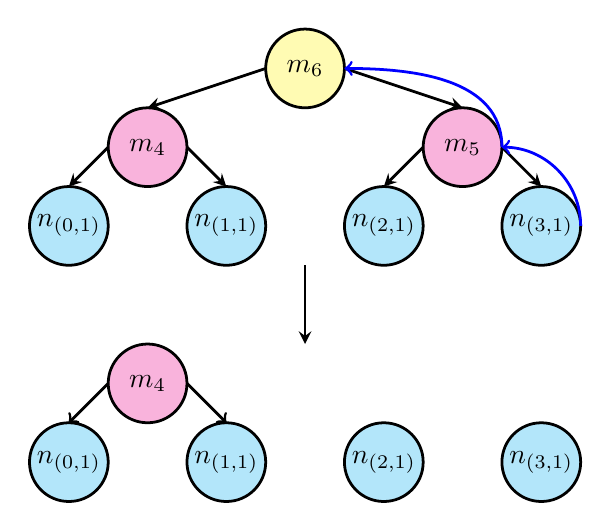
\begin{tikzpicture}[scale=0.5] % Adjust the scale factor as needed
        % Your TikZ code goes here
        \draw[line width=1pt,fill=yellow!30] (0,0) circle (1cm);
        \node at (0,0) {$m_6$};
        \draw[line width=1pt, fill=magenta!30] (-4,-2) circle (1cm);
        \node at (-4,-2) {$m_4$};
        \draw[line width=1pt, fill=magenta!30] (4,-2) circle (1cm);
        \node at (4,-2) {$m_5$};
        \draw[line width=1pt, fill=cyan!30] (-6,-4) circle (1cm);
        \node at (-6,-4) {$n_{(0,1)}$};
        \draw[line width=1pt, fill=cyan!30] (-2,-4) circle (1cm);
        \node at (-2,-4) {$n_{(1,1)}$};
        \draw[line width=1pt, fill=cyan!30] (6,-4) circle (1cm);
        \node at (6,-4) {$n_{(3,1)}$};
        \draw[line width=1pt, fill=cyan!30] (2,-4) circle (1cm);
        \node at (2,-4) {$n_{(2,1)}$};
        \draw[-> , >=stealth,line width=1pt] ({0 + cos(180)},{0 + sin(180)}) -- (-4,-1);
        \draw[->, >=stealth, line width=1pt] ({0 + cos(0)},{0 + sin(0)}) -- (4,-1);
        \draw[->, >=stealth, line width=1pt] ({-4 + cos(180)},{-2 + sin(180)}) -- (-6,-3);
        \draw[->, >=stealth, line width=1pt] ({-4 + cos(0)},{-2 + sin(0)}) -- (-2,-3);
        \draw[->, >=stealth, line width=1pt] ({4 + cos(180)},{-2 + sin(180)}) -- (2,-3);
        \draw[->, >=stealth, line width=1pt] ({4 + cos(0)},{-2 + sin(0)}) -- (6,-3);
        
        % Curved arrow
        \draw[->, color=blue, line width=1pt] (7, -4) to[out=90, in=0] (5, -2);
        \draw[->, color=blue, line width=1pt] (5, -2) to[out=90, in=0] (1, 0);
        \draw[->, >=stealth, line width=1pt] (0,-5) to (0,-7);

        \draw[line width=1pt, fill=magenta!30] (-4,-8) circle (1cm);
        \node at (-4,-8) {$m_4$};
        \draw[line width=1pt, fill=cyan!30] (-6,-10) circle (1cm);
        \node at (-6,-10) {$n_{(0,1)}$};
        \draw[line width=1pt, fill=cyan!30] (-2,-10) circle (1cm);
        \node at (-2,-10) {$n_{(1,1)}$};
        \draw[line width=1pt, fill=cyan!30] (6,-10) circle (1cm);
        \node at (6,-10) {$n_{(3,1)}$};
        \draw[line width=1pt, fill=cyan!30] (2,-10) circle (1cm);
        \node at (2,-10) {$n_{(2,1)}$};
    
        \draw[->, line width=1pt] ({-4 + cos(180)},{-8 + sin(180)}) -- (-6,-9);
        \draw[->, line width=1pt] ({-4 + cos(0)},{-8 + sin(0)}) -- (-2,-9);

    \end{tikzpicture}
    \caption{Trees and Cuts}
    \label{fig:Order_of_merging}
\end{figure}


In our abstraction refinement loop, we start with the fully merged network.
Then, whenever we get a \gencex $\vct{\beta}$ (Section \ref{s:qual}), we wish to
refine the network, that is, we wish to chose which
neurons should remain merged. Intuitively, this choice should be guided
two factors: optimising with respect to the semantic behavior of the network,
and attempting to eliminate $\vct{\beta}$.

The tree produced in the previous Section \ref{s:tree} captures the semantic
behavior, and we use it to guide the refinement process as follows:
Any cut of the tree produces a set of trees. Then,  
the groups of neurons that we chose to keep merged correspond to the leaf nodes
of the  these trees. Therefore finding a refinement is reduces to finding a cuts
in the tree.

To attempt to eliminate $\vct{\beta}$, we identify a \textit{culprit neuron}
$\gamma$ that contributes most to the spurious output on $\vct{\beta}$. The
intuition is that $\gamma$ should not be merged with any other neuron, as any
over-approximation of the behavior of $\gamma$ has a high chance of
introducing $\vct{\beta}$.

Thus, we do refinement in two steps. Firstly we find the culprit neuron
$\gamma$. Then, we find a cut in the tree that ensures that $\gamma$ is not
merged with any other neuron.

\subsubsection{Finding $\gamma$}

Many possible heuristics may be used to identify the culprit neuron $\gamma$,
and our framework is agnostic to the specific heuristic chosen. In this work, we
use a heuristic based on the 'gradient-guided refinement' described in
\cite{lin-comb-abs-jan}. A neuron is designated as the culprit neuron $\gamma$
when the following value is maximum for that neuron: 

\begin{equation*}
\begin{aligned}
    \|v^{*}_{\gamma}(\vct{\beta}) - v_{\gamma}(\vct{\beta})\|_{2} \cdot 
    \big| \frac{\delta y(\vct{\beta})}{\delta v_{\gamma}} \big|
\end{aligned}
\end{equation*}

Here, $v_{\gamma}(\vct{\beta})$ is the value at the neuron $\gamma$ for input
$\vct{\beta}$ in the original \cnc, while $v^{*}_{\gamma}(\vct{\beta})$ is the
value of the neuron $\gamma$ has been merged to in our current \abs.
$\frac{\delta y(\vct{\beta})}{\delta v_{\gamma}}$ is the gradient of the output
$y$ of \cnc with respect to the value at $\gamma$ for the input $\vct{\beta}$.

\subsubsection{Cutting the Tree}

We wish to find a cut in the tree where $\gamma$ is not merged to any other
neuron, while also making sure that as many neurons remain merged as possible
(therefore minimizing the increase in size of \abs). To do this, we delete
precisely those nodes that are dependent on $\gamma$, starting form the parent
of $\gamma$ and moving up the tree following the parent of each.

Once we have cut the tree and decided on which neurons to leave merged, the
actual merge operation is the exact same as that followed by \cite{cegar-nn}
(Section \ref{s:nn-sam}). Therefore, we are able to retain concrete soundness
guarantees.

In our example, the culprit neuron is $\nr{1}{3}$. Thus, we traverse the tree
following the blue edges Figure \ref{fig:Order_of_merging}, undoing $m_5$ and
$m_6$. This produces three trees, corresponding to leaving $\nr{1}{0}$ and
$\nr{1}{1}$ merged, while undoing the merge of $\nr{1}{2}$ and $\nr{1}{3}$.
Therefore, we get the \abs shown in Figure \ref{fig:tree_cut_refine}. Note
that in contrast to the refinement process followed by \cite{cegar-nn} (Section
\ref{s:nn-sam}), we retain merges of neurons that are semantically close, avoid
proliferation of singletons and achieve a smaller \abs that is sufficient to
prove the property in fewer iterations.

\begin{figure}[htbp]
    \centering
    \begin{tikzpicture}[scale=0.5] % Adjust the scale factor as needed
      % Your TikZ code goes here
      \draw[fill=blue!30, line width = 1pt] (0,2) circle (1cm);
      \node at (0,2) {$n_{(0,0)}$};
      \node [text=red] at (-2,2) {1};
      \draw[fill=blue!30, line width = 1pt] (0,-2) circle (1cm);
      \node [text=red] at (-2,-2) {1};
      \node at (0,-2) {$n_{(1,0)}$};
      \draw[fill=orange!30, line width = 1pt] (5,4) circle (1cm);
      \node at (5,4) {$m_4$};
      \node [text=red] at (5,2.5) {1.5};
      \draw[fill=pink!30, line width = 1pt] (5,-4) circle (1cm);
      \node at (5,-4) {$n_{(3,1)}$};
      \node [text=red] at (5,-5.5) {1.5};
      \draw[fill=pink!30, line width = 1pt] (5,0) circle (1cm);
      \node at (5,0) {$n_{(2,1)}$};
      \node [text=red] at (5,-1.5) {1.9};
      \draw[fill=green!30, line width = 1pt] (10,0) circle (1cm);
      \node at (10,0) {$n_{(0,2)}$};
      \node [text=red] at (12,0) {$6.8$};
    \draw[->, >= angle 45, line width = 1pt, postaction={decorate, decoration={text along path, 
    text={0.55}, text align=center, raise=1mm}}](1, 2) -- (4, 4);
    \draw[->,>= angle 45, line width = 1pt] (1, -2) to (4, 4);
    \node at (3.75,3) {1};
    \draw[->,>= angle 45, line width = 1pt](1, 2) -- (4, 0);
    \node at (3.75,1) {0.95};
    \draw[->,>= angle 45, line width = 1pt](1, -2) -- (4, 0);
    \node at (3.75,-1) {0.55};
    \draw[->,>= angle 45, line width = 1pt](1, 2) -- (4, -4);
    \node at (3.75,-3) {1};
    \draw[->, >= angle 45, line width = 1pt, postaction={decorate, decoration={text along path, 
    text={0.5}, text align=center, raise=1mm}}](1, -2) -- (4, -4);
    \draw[-> , >= angle 45, line width = 1pt, postaction={decorate, decoration={text along path,
    text={1}, text align=center, raise=1mm}}] (6,-4) -- (9, 0);
    \draw[->, >= angle 45, line width = 1pt, postaction={decorate, decoration={text along path,
    text={1}, text align=center, raise=1mm}}] (6,0) -- (9, 0);
    \draw[->, >= angle 45, line width = 1pt, postaction={decorate, decoration={text along path,
    text={2}, text align=center, raise=1mm}}] (6,4) -- (9, 0);
   
    % \draw (1, -2) -- (4, 2);
    % \node at (3.75,1.25) {1};
  
    % \draw (1, 2) -- (4, -2);
    % \node at (3.75,-1.25) {1};
  
    % \draw[solid, postaction={decorate, decoration={text along path,
    % text={0.95}, text align=center, raise=1mm}}] (1, 2) -- (4, 2);
   


    % \draw[solid, postaction={decorate, decoration={text along path,
    % text={1}, text align=center, raise=1mm}}] (6,-2) -- (9, 0);
    % \draw[solid, postaction={decorate, decoration={text along path,
    % text={3}, text align=center, raise=1mm}}] (6, 2) -- (9, 0);

    \end{tikzpicture}
    \caption{Refining by our method: Culprit Neuron is 3 }
    \label{fig:tree_cut_refine}
  \end{figure}
  


\subsection{Optimality of Tree}
\label{s:optimal-tree}

The tree $T$ produced in Section \ref{s:tree} captures an optimal ordering of
merge operations with respect to the semantic information in the following
sense:

Let $T_1$ and $T_2$ be two sub-trees of $T$. Then, the maximum value of $\cls$
for any two neurons that are leaves $T_1$ (or $T_2$) is smaller than the maximum
value of $\cls$ for any two neurons one from $T_1$ and another from $T_2$.
\dmcmt{Make this a lemma?}

This fact can be easily proved via induction on the combined size of $T_1$ and
$T_2$ \todo{Ref appendix}. Note that this proof crucially depends on the fact
that we took pairwise maximum in Algorithm \ref{a:build-tree} in Section
\ref{s:tree}.

Thus, we have that for any cut in the tree, the
maximum difference in the semantic behavior for neurons that have been left
merged is less than the maximum difference in semantic behavior for neurons that
have been un-merged. In particular, this implies that after each refinement
step, the groups of neurons that remain merged together are optimal with respect
to the semantic behavior of the network.

\dmcmt{Since semantic closeness doesn't actually anything concrete and
    quantitative about what happens at the output, this optimality is not able
to claim anything about output values. Discuss this? Bringing this up may invite
more questions, and so an appropriate discussion may take too much space...}

\subsection{General Abstraction-Refinement Loop}
\label{s:abs-ref-fw}

We combine the pieces discussed so far into an abstraction-refinement loop. The
exact arrangement of the loop depends on the particular application, but the
general structure is as follows:

We start with the fully merged network. Then, utilising \gencex, we iteratively
refine the network until we have obtained an \abs with the desired quality.

Depending on the application, the \gencex used for refinement may come from
several places, and our framework is agnostic to this. For example, when solving
a neural network query, it may be a spurious counterexample returned by a solver
call, in which case our general abstraction-refinement loop reduces to a
standard CEGAR loop. On the other hand, when attempting to produce a safe
compression (Section \ref{s:exp-mnist-comp}), the \gencex may come form a false
positive classification on a training dataset.
